\chapter*{Annexes}

Before creating functions,we imported different libraries.
\begin{figure}[bth]%[!ht]
\begin{center}
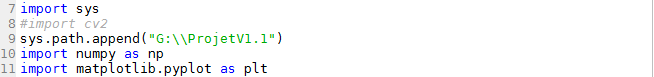
\includegraphics[scale=0.75]{import_bibliotheque}%[height=70mm,width=70mm]
%\caption{\textbf{jbbv}}%
%\url {http://www.google.fr/}
\label{read_}%
\end {center}
\end{figure}
\\The module sys gives direct acces to the arguments of the command line.
\\The module numpy is a digital library providing efficient support for large multidimensional arrays,and high-level mathematical funtiuns as linear algebra,statistics ...
\\The module Matplotlib is a library programming language that combined with python library numpy and scipy is a powerfull tool for tracing and visualizing data.
\section{Eigenfaces functions}
In this part ,we will put the different functions and their explenations
\begin{itemize}
\item Function used to load  images from directories
\begin{figure}[bth]%[!ht]
\begin{center}
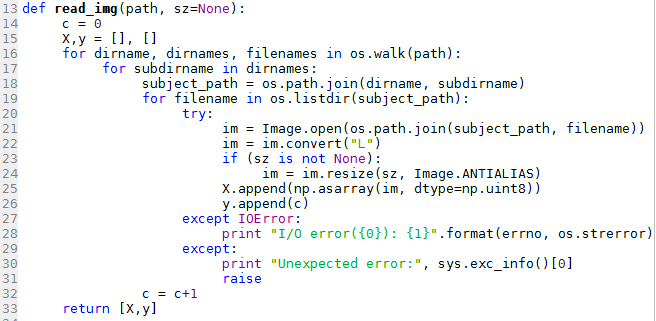
\includegraphics[scale=0.75]{fonc_ReadImg}%[height=70mm,width=70mm]
%\caption{\textbf{jbbv}}%
%\url {http://www.google.fr/}
\label{read_}%
\end {center}
\end{figure}
\\This function has input the full path to load all the images of the database.
It returns X which is a list of all the combined images and y which is the subscript i of all images for the subject i.
%\paragraph{}
\newpage
\paragraph{}
\item  Function used to transform matrix to vector
\begin{figure}[bth]%[!ht]
\begin{center}
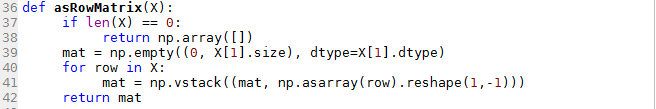
\includegraphics[scale=0.75]{fonc_marixVectors}%[height=70mm,width=70mm]
%\caption{\textbf{jbbv}}%
%\url {http://www.google.fr/}
\label{read_}%
\end {center}
\end{figure}
\\This function transforms an  images matrix  as a vector. It takes as input a matrix A and returns a vector mat.
\\The function vstack   returns  an vertical vector.
\paragraph{}
\item Function for calculating the average and centering all images
\begin{figure}[bth]%[!ht]
\begin{center}
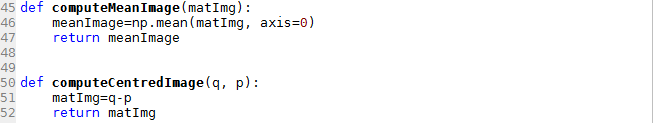
\includegraphics[scale=0.75]{fonc_mean_and_centred_img}%[height=70mm,width=70mm]
%\caption{\textbf{jbbv}}%
%\url {http://www.google.fr/}
\label{read_}%
\end {center}
\end{figure}
\\The function ComputeMeanImage takes as input the  matrix matImg and returns the average image for the  learning base.
\\ The function ComputeCentredImage center each image .The  average image is subtracted from each image
\\It returns back matIm:corresponding to the result of the image centered.
\item The function for calculating the covariance matrix
\begin{figure}[bth]%[!ht]
\begin{center}
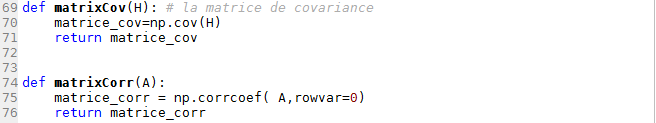
\includegraphics[scale=0.75]{fonc_matrix_cov_and_corr}%[height=70mm,width=70mm]
%\caption{\textbf{jbbv}}%
%\url {http://www.google.fr/}
\label{read_}%
\end {center}
\end{figure}
\\corrcoef  standardize the covariance matrix.
\newpage
\item Functions for calculating specific elements
\begin{figure}[bth]%[!ht]
\begin{center}
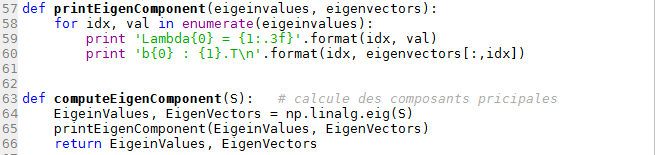
\includegraphics[scale=0.75]{fonc_print_and_compute_eigenvector_eigenvalue}%[height=70mm,width=70mm]
%\caption{\textbf{jbbv}}%
%\url {http://www.google.fr/}
%\label{read_}
\end {center}
\end{figure}
%\paragraph{}
\\The function printEigenComponent print eigenvalues and eigenvectors.
\\The function computeEigenComponent calculates  eigenvalues and eigenvectors. They are computed with the normalized covariance matrix.
\paragraph{}
\item Main funtion gathering invocation of other computing functions 
\begin{figure}[bth]%[!ht]
\begin{center}
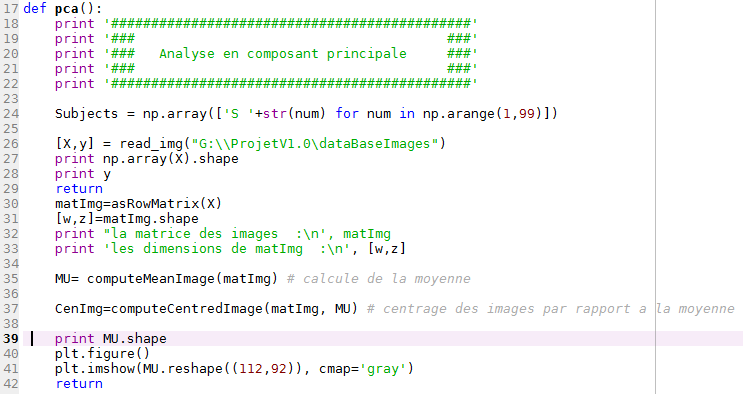
\includegraphics[scale=0.75]{affich_MeanImg}%[height=70mm,width=70mm]
%\caption{\textbf{jbbv}}%
%\url {http://www.google.fr/}
%\label{read_}
\end {center}
\end{figure}
\\This function allows to call others functions and create projection axes of eigenvectors and we also saved the average image.
%\clearpage
%\begin{figure}[bth]%[!ht]
%\begin{center}
%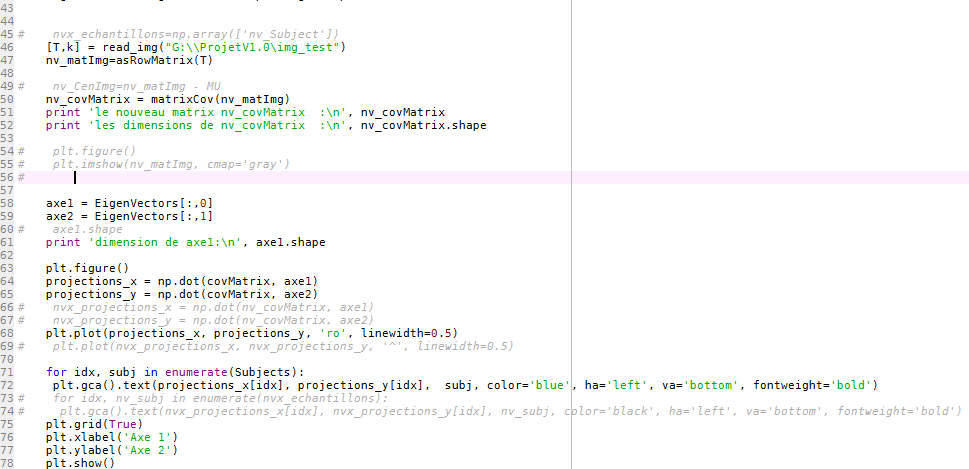
\includegraphics[scale=0.75]{fonction_pca1}%[height=70mm,width=70mm]
%\caption{\textbf{jbbv}}%
%\url {http://www.google.fr/}
%\label{read_}
%\end {center}
%\end{figure}
%\paragraph{}


\end{itemize}


